\chapter{Evaluation}

\section{Introduction}

\begin{itemize}
    \item Talk about why the three sections below are being talked about
\end{itemize}


\section{Interconnect Performance}

Calling a function implemented in hardware off-chip is not latency free. There will be some overhead latency associated with packaging the data to be sent over the channel, sending the data over the channel itself, and then repeating this process in order to return the data produced by the off-chip function back to the main FPGA. Therefore, it is of importance to measure this overhead so that we can gauge the efficiency of the interconnect hardware that was designed for SystemNaim.

Since the decision was made to implement an SPI communication channel for the final product, we had to into consideration the SPI clock speed used by the system. On an SPI channel, a single bit is sent on every cycle of the SPI clock meaning it takes 32 SPI Clock cycles to send single 32-bit integer. Increasing the SPI Clock speed allows for a higher performing channel, which is able to send data in a shorter period, however, this increase comes at the cost of reliability. This section explores the effect of the SPI Clock rate on a test system. We will attempt to prove that increasing the clock speed does reduce the total overhead, but will also investigate the overhead added from the interconnect to the latency of the system.

\subsection{Test Model}

In order to find out how much of the latency of a multi-FPGA system, created in SystemNaim, can be attributed to the interconnect, we must first devise a model that can tell us what data needs to be gathered. At it's most simple, we can model the latency of a system as the sum of the time taken to perform the actual processing i.e. the code that the user entered into the tool, and the time taken to encode, transmit, receive, and decode the data across the SPI channel i.e. the overhead. \autoref{eqn:tot_sys_latency}, shows the mathematical equivalent of the previous statement.

\begin{equation}
    L_{sys} = L_{processing} + L_{overhead}
    \label{eqn:tot_sys_latency}
\end{equation}

In order to find $L_{processing}$ from \autoref{eqn:tot_sys_latency} we make the following assumption: the total processing time, in cycles, for a multi-FPGA system is the same as a single FPGA system where both the off-chip function and on-chip function, from the former system, are run in parallel. In essence, if measure the latency of a system that has been created on a single FGPA using SystemNaim's “split” keyword then we can assume the total latency of this system is equal to $L_{processing}$ for a multi-FPGA system where “split” has been replaced with “split-fpga”.

Before we continue an important side note, $L_{rest}$ will refer to the latency caused by the processing outside the function call i.e. the processing before and after the function call. In terms of hardware SystemNaim generates the exact same in both the single FPGA and multi-FPGA case before and after the function call. Furthermore, for simplicity the single FPGA system with parallel hardware will be called the Multi-Thread Single Chip (MTSC) system, as it denotes parallel computation on a single chip, likewise, the multi-FPGA system will be referred to as the Multi-Thread Multi-Chip (MTMC) system. 

We can prove that $L_{processing} = L_{MTSC}$, where $L_{MTSC}$ is the total latency for an MTSC system, if we place the following constraint on the system: all parallel function in the system must have the same latency.

\autoref{fig:multi_func_call} is a diagram representing the program path for a multi-function call a MTSC system. As can be seen the total latency $L_f = max(L_1,L_2)$, however with our constraint $L_1 = L_2$, and thus we can simplify to \autoref{eqn:fcl_2}. \autoref{fig:multi_fpga_call} shows a similar diagram for the MTMC case. Assuming both functions are the same and that $L_{I1} > 0 \&\& L_{I2} > 0 $ then equations \ref{eqn:mtmc_latency_start} to \ref{eqn:mtmc_latency} hold. 

\begin{align}
    &L_{f\_MTSC} = L_1 \label{eqn:fcl_1} \\
    &L_{MTSC} = L_{rest} + L_1 \label{eqn:fcl_2}
\end{align}

\begin{align}
    &L_{f\_MTMC} = max(L_1 + L_{I1} + L_{I2} , L_2) = L_1 + L_{I1} + L_{I2} \label{eqn:mtmc_latency_start} \\
    &L_{MTMC} = L_{rest} + L_1 + L_{I1} + L_{I2}  \\
    &L_{MTMC} = L_{MTSC} + L_{I1} + L_{I2} \\
    \therefore \; &L_{processing} = L_{MTSC} \label{eqn:mtsc_processing} \\
    \& \; &L_{overhead} = L_{I1} + L_{I2} 
    \label{eqn:mtmc_latency}
\end{align}

Finally, given those results we prove that we can use the MTSC latency in the MTMC calculations. We also proved that the overhead was $L_{overhead} = L_{I1} + L_{I2}$, which represent the latency incurred by sending and receiving data, respectively, and seems like a sensible conclusion. Furthermore, \autoref{eqn:overhead_formula} show's that we can calculate the overhead latency by finding the difference between the latency of an MTMC and MTSC system, provided that they both call the same functions and have the same processing before and after the function call. In SystemNaim this is easily doable by switching the “split” keyword with “split-fpga”. 

\begin{align}
    &L_{MTMC} = L_{processing} + L_{overhead} \\
    &L_{overhead} = L_{MTMC} - L_{processing}  \\
    &L_{overhead} = L_{MTMC} - L_{MTSC}\label{eqn:overhead_formula}
\end{align}

\begin{figure}[!htb]
    \centering
    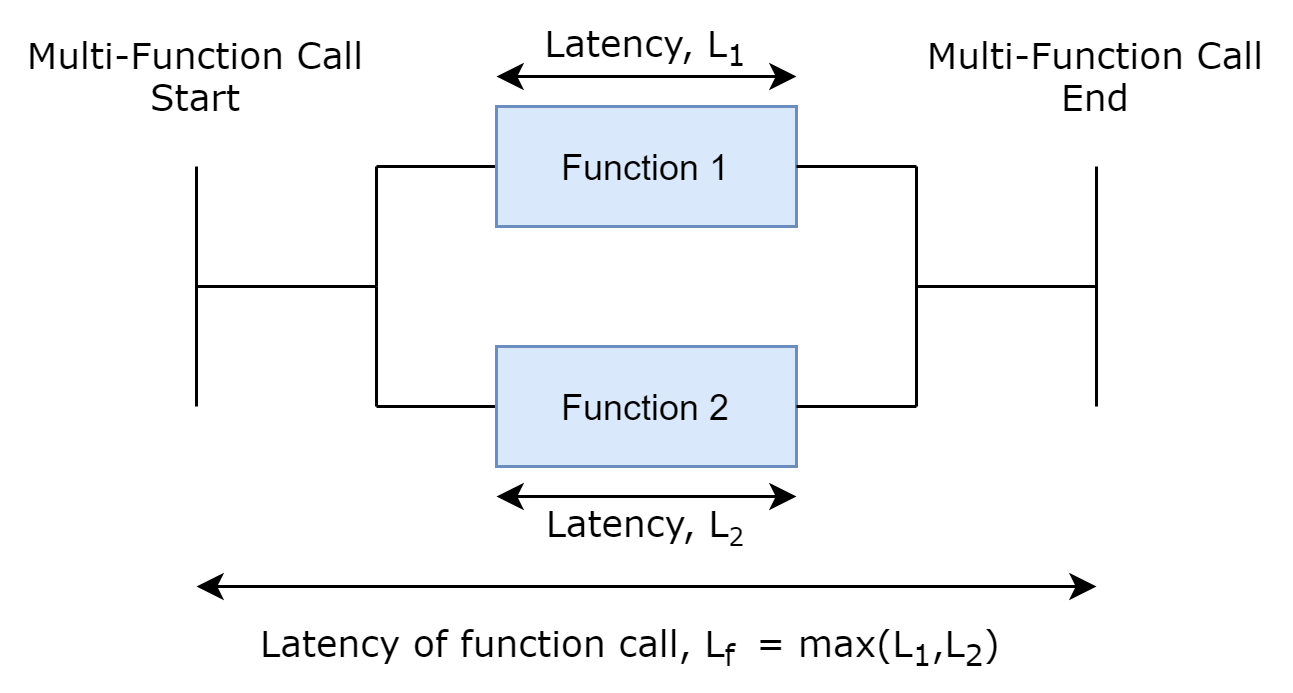
\includegraphics[width=0.9\textwidth]{05_evaluation/images/concurrent_latency.png}
    \caption{Latency of single FPGA multi-function call}
    \label{fig:multi_func_call}
\end{figure}

\begin{figure}[!htb]
    \centering
    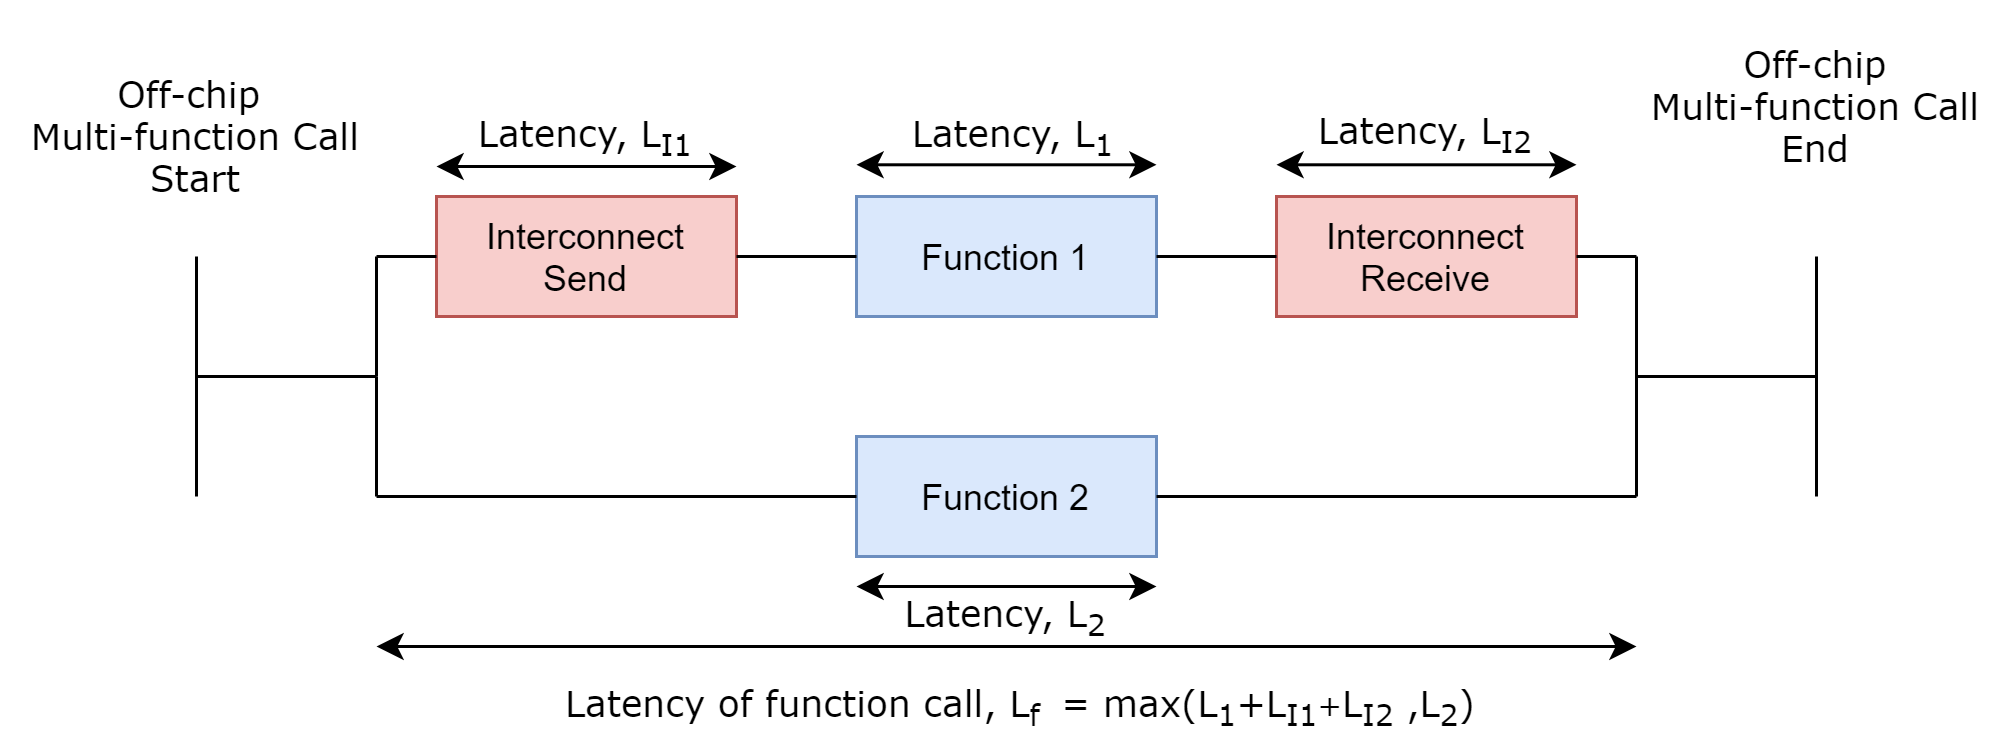
\includegraphics[width=0.9\textwidth]{05_evaluation/images/offchip_latency.png}
    \caption{Latency of multi FPGA multi-function call}
    \label{fig:multi_fpga_call}
\end{figure}

\subsection{Channel Bandwidth}
 
We can further dissect the overhead latency and split it into two parts. The transfer overhead, $L_{t\_overhead}$, which is latency cost incurred for transmitting and receiving data over a channel and the interconnect overhead, $L_{i\_overhead}$, which is the latency cost from encoding and decoding the data transmitted. Essentially, the latter part comes from the hardware designed specifically for SystemNaim, whereas the former is merely the limit of the channel. In an ideal world the interconnect overhead would be 0 and only the transfer overhead would exist. 

We can calculate the transfer overhead by knowing the rate at which data is transferred over the channel, in the case of an SPI channel this is dependent on the SPI clock speed, $\mathit{SPI}_{clock}$. The SPI clock speed is different from the system clock speed, $\mathit{SYS}_{clock}$, both can be configured by the user but in our case we have a variable SPI clock speed and a static system clock speed at 50MHz.

Our SPI channel transfers data at 1 bit per SPI clock cycle, which is standard, however we're not interested in how long it takes for data to be transferred relative to the SPI clock. Instead, we would like to know how many system clock cycles it takes to transmit a single bit. We'll refer to this value as the channel latency, $L_{channel}$, and it can be calculated by dividing the system clock speed by the SPI clock speed. The resulting value has a unit of cycles per bit.

For SystemNaim, we know that any off-chip function call requires 128 bits of data to be sent over the channel. 96 bits (or 3 integers) are required to send the opcode, operand A and operand B, while the last 32 bits are for the data that needs to be returned to the main FPGA. Therefore, the formula for the transfer overhead, which is measure of how many clock cycles it takes to transfer all the data over a channel for an off-chip function call, is shown in \autoref{eqn:overhead}. 

\begin{equation}
    L_{channel} = \frac{\mathit{SYS}_{clock}}{\mathit{SPI}_{clock}} 
    \label{eqn:clock_speed}
\end{equation}

\begin{equation}
    L_{t\_overhead} = 128 * L_{channel}
    \label{eqn:overhead}
\end{equation}

\subsection{Testing}

With the maths and the modelling in place we can now being testing the system to see if we can get an experimental value for the overhead and how it is affected by the SPI clock speed. For this test we use a program which calls 2 function, which are syntactically the same, and then exits. We first compile program with both functions be called within a “split” block and test the latency of this MTSC system. Afterwards we test the same program, but we replace the “split” keyword with the “split-fpga” keyword, this will be the MTMC system. 

The MTMC system will be run multiple times with varying SPI clock speeds, and for each test we will compare the latencies between the MTMC and MTSC systems, compute the transfer overhead and find the interconnect overhead.

\subsection{Results}

\autoref{tbl:spi_clk_results} shows the data gathered, in accordance to testing methodology laid out above. It should be noted that the \textbf{Channel Latency} and \textbf{Est. Transfer Overhead} columns have been calculated using no gathered data. Both columns are dependent on the \textbf{SPI Clock (Hz)}, and the calculations for each can be found in Equation \ref{eqn:clock_speed} and \ref{eqn:overhead} respectively.

\autoref{fig:spi_clk_graph} is a summation of the important data from the table in the form of graph, thus making it easier to identify trends in the data.

\begin{sidewaystable}
    \centering
    \begin{threeparttable}
    \begin{tabular}{l|l|l|l|l|l}
    \textbf{SPI Clock (Hz)} & \textbf{Channel Latency} & \textbf{Latency (Cycles)} & \textbf{Overhead (Cycles)} & \textbf{Transfer Overhead} & \textbf{Interconnect Overhead} \\ \hline
     125,000               &  400                 &  52,918              &  52,794              & 51,200                &  1,594                                      \\
     250,000               &  200                 &  26,518              &  26,394              & 25,600                &  794                                        \\
     252,525\tnote{*}      &  198                 &  26,254              &  26,130              & 25,344                &  786                                        \\
     277,777\tnote{*}      &  180                 &  23,878              &  23,754              & 23,040                &  714                                        \\
     312,500               &  160                 &  26,532              &  26,408              & 20,480                &  5,928                                      \\
     347,222\tnote{*}      &  144                 &  23,892              &  23,768              & 18,432                &  5,336                                      \\
     500,000               &  100                 &  16,632              &  16,508              & 12,800                &  3,708                                      \\
     1,000,000             &  50                  &  8,382               &  8,258               & 6,400                 &  1,858                                      \\
     1,923,076\tnote{*}    &  26                  &  4,422               &  4,298               & 3,328                 &  970                                        \\
     5,000,000             &  10                  &  1,782               &  1,558               & 1,280                 &  278                                        \\
     8,333,333\tnote{*}    &  6                   &  1,122               &  998                 & 768                   &  230                                        \\
     12,500,000            &  4                   &  792                 &  668                 & 512                   &  156                                        \\
     25,000,000            &  2                   &  542                 &  418                 & 256                   &  162                                       
    \end{tabular}
    \begin{tablenotes}\footnotesize
        \item[*] These values for SPI clock speed are not factors of the system clock, and are actually irrational.
        \end{tablenotes}
    \end{threeparttable}
    \caption{Effect of SPI clock speeds on overhead latency}
    \label{tbl:spi_clk_results}
\end{sidewaystable}

\begin{figure}[!htb]
    \centering
    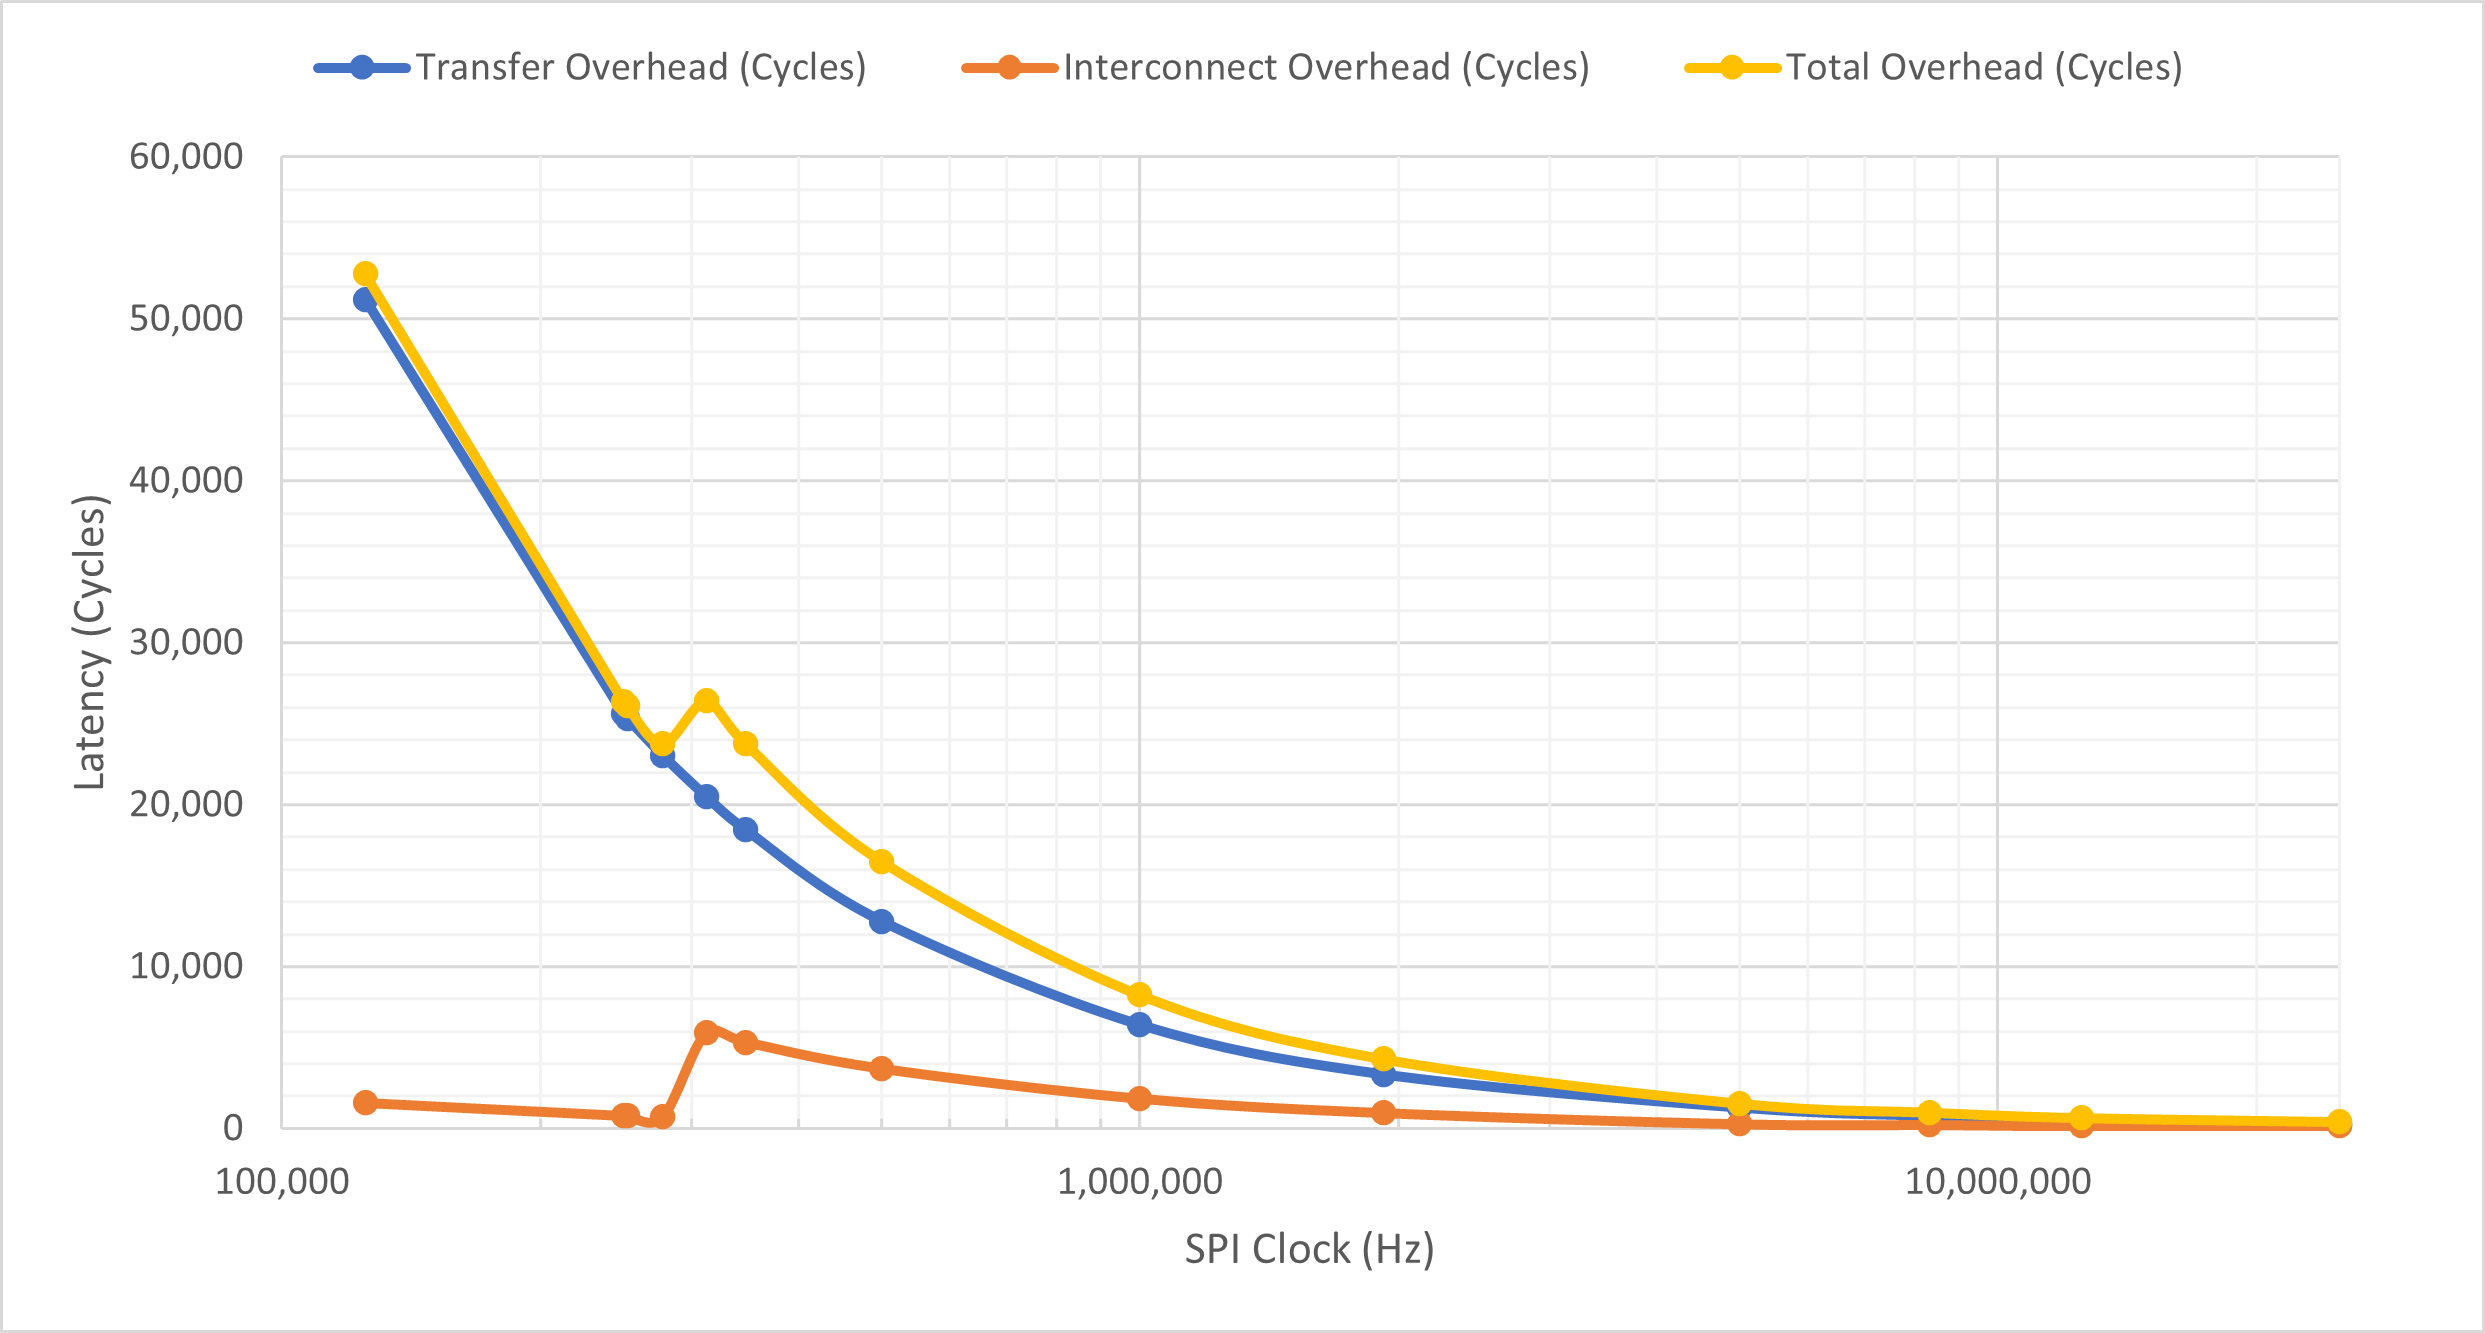
\includegraphics[width=0.9\textwidth]{05_evaluation/images/overhead_vs_spi_clk.png}
    \caption{Overhead Latency vs. SPI Clock Speed}
    \label{fig:spi_clk_graph}
\end{figure}


\subsection{Conclusions}

Generally speaking, we can conclude that as we increase the SPI clock speed the total overhead latency decreases aswell as that the main proportion of the overhead is transfer overhead. This is supported by \autoref{fig:spi_clk_graph}, and was the result we intended for this investigation to prove. However, there are a few interesting caveats to this conclusion that we cannot ignore. Firstly, while not shown on the graph or table, during testing it was found that setting the clock speed the values higher than 8MHz resulted in increased channel instability. Tests would occasionally fail to complete with transactions not being detected by either the on-chip or off-chip interconnect, the higher the clock speed the more likely this phenomenon would occur.

This instability may have been caused by the physical components of the channel not being able to accurately keep up with these speeds. For the final product GPIO pins on both FPGAs were connected using breadboard jumper cables, which aren't intended to be used for data communication. Potentially, at clock speeds of 8MHz and above, the GPIO pins were not able to go from high to low, and vice versa, fast enough to generate a detectable clock on the child FPGA. The fault could also lie with the SPI core and the FPGA hardware. The SPI core takes in the main system clock, generates the SPI Clock and transmits that signal to a GPIO pin. Therefore, there may be an issue at the hardware level between the pin and the FPGA hardware. Unfortunately, there's no way to be certain of the cause, and instead we can only conclude that speeds above 8MHz result in unreliable performance. 

The more interesting result from the gathered data, however, comes from the trend of the \textbf{Interconnect Overhead}. While it would be expected that the latency from the interconnect would be generally static, with only minor fluctuations, since the task of encoding data should be uniform, what we see instead is a generally decreasing trend except for a steep rise in latency at 312,500Hz. This behaviour, however, makes complete sense given the design of the interconnect and is a consequence of the SPI channel only allowing the master to initiate transactions. 

As explained in SOME IMPLEMENTATION SECTION, the child FPGA cannot indicate to the parent FPGA when it has completed processing its off-chip function. Therefore, in order to receive the return data the parent FPGA must continuously send polling transactions on the SPI channel. When any transaction is started by the master SPI core on the parent FPGA, the slave SPI core starts simultaneously transmitting data stored in an internal register. At some point during operation, this internal register will contain the result of the off-chip function call, but that point cannot be determined beforehand and thus arises the need for continuous polling transactions, a diagram of this process is shown in \autoref{fig:interconnect_polling}. Because of this, when the off-chip function is complete, and it passes the result to the SPI slave core, the core must wait for the current polling transaction to finish before the next one starts, and then it can send the valid return data. Therein lies the issue, the wait for a current transaction to finish.

The worst case for this scenario is if the slave SPI core has to wait for a full transaction, minus one cycle, to complete before it can send its data. At lower clock rates this can take thousands of cycles, more specifically $32 * L_channel$ cycles, since each transaction consists of 32 bits. Furthermore, how close the end time of an off-chip function is to the end of any given polling transaction is dependent on both the SPI clock speed and the latency of the function itself, therefore it becomes incredibly difficult to avoid the worse case scenario and the interconnect overhead becomes a stochastic model. However, we can minimize the interconnect overhead by increasing the SPI clock speed, as this reduces the number of system cycles it takes for a polling transaction to finish and thus also the number of system cycles the slave SPI core has to wait in the worse case scenario.

In conclusion, we should try to maximize the SPI clock speed as this reduces the transfer overhead, and minimizes the worst case for the interconnect overhead, thus, increasing the performance of the MTMC system.


\begin{figure}[!htb]
    \centering
    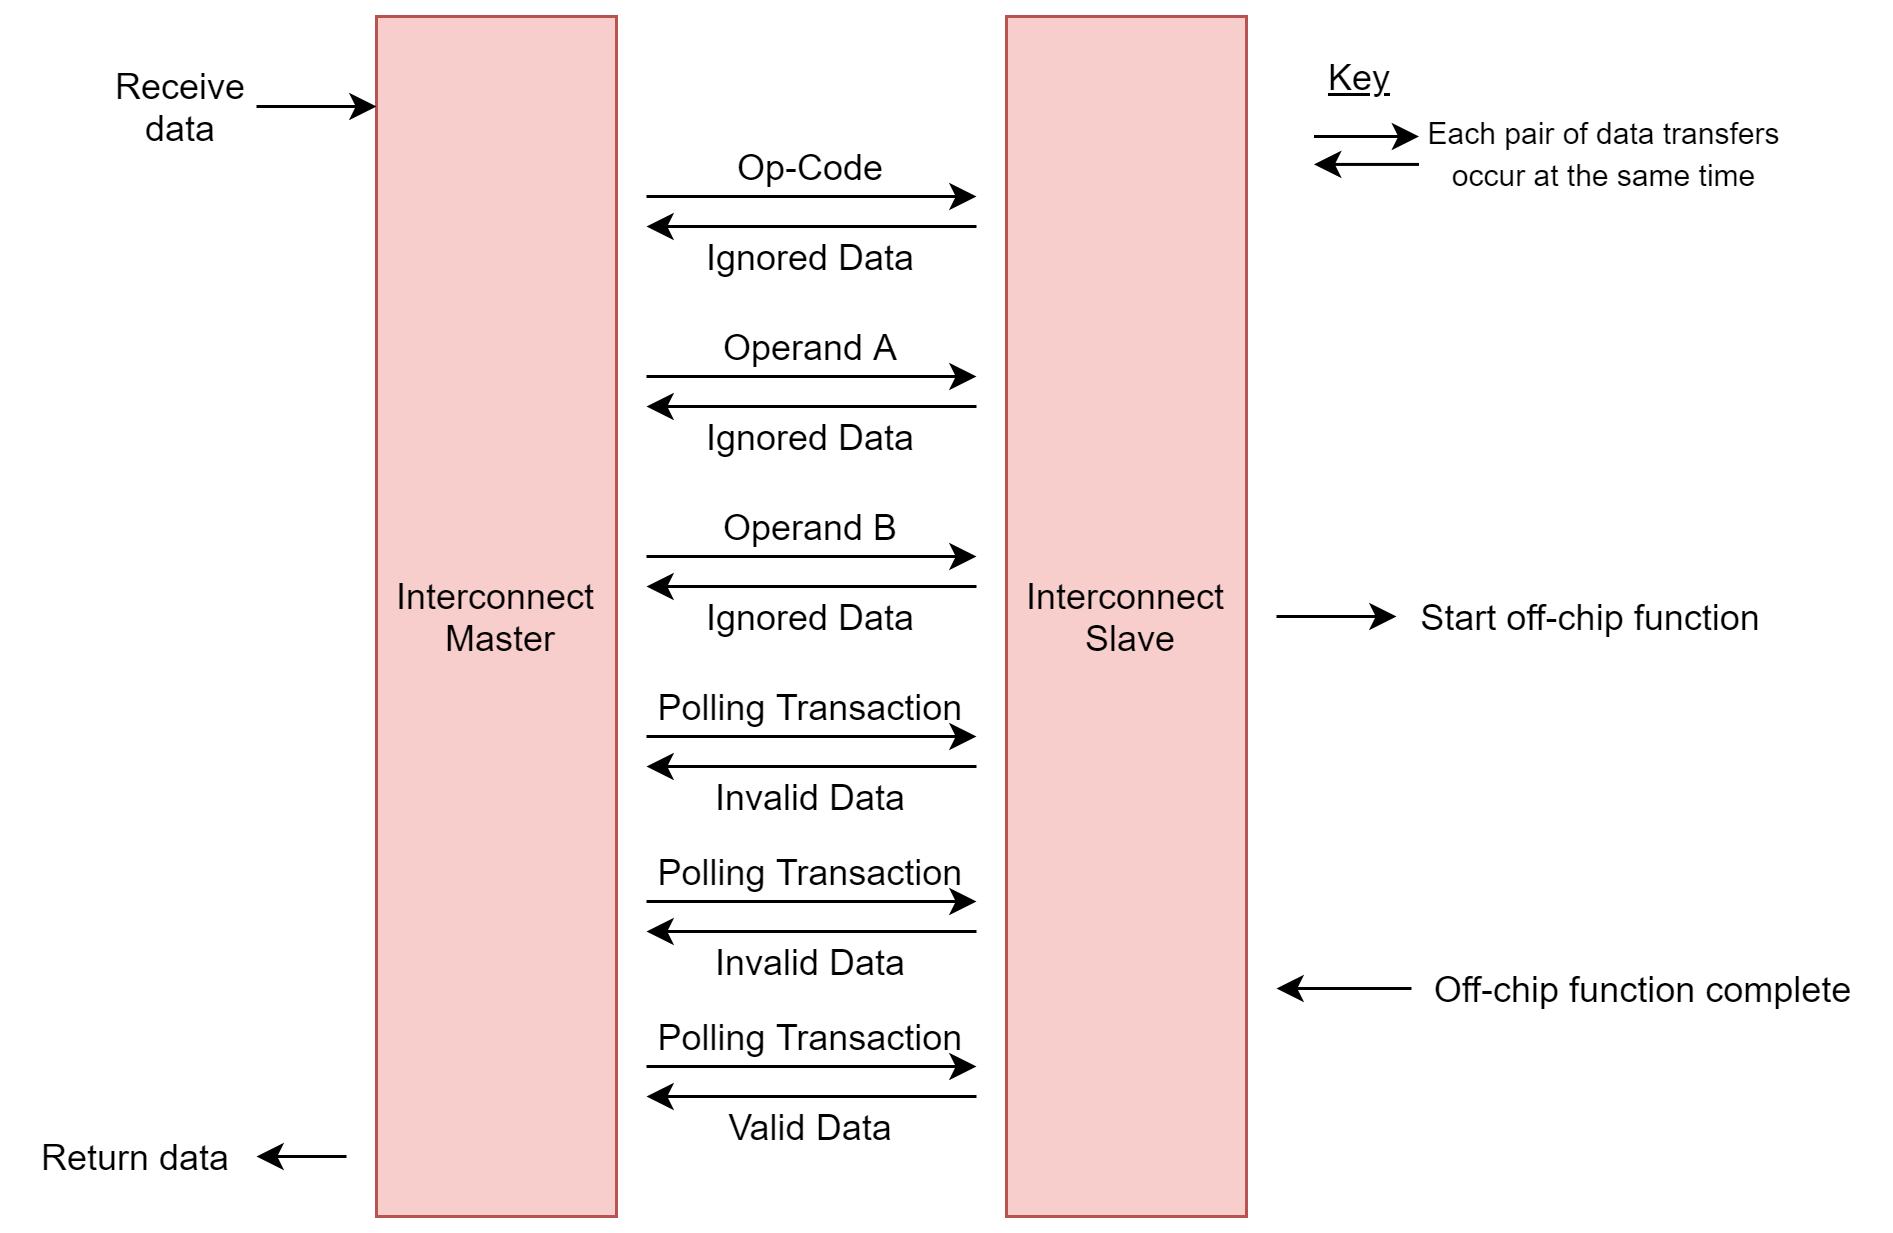
\includegraphics[width=0.9\textwidth]{05_evaluation/images/interconnect_polling.png}
    \caption{Example of interconnect communication protocol in practice}
    \label{fig:interconnect_polling}
\end{figure}


\section{System Performance}

\begin{itemize}
    \item This section goes over how much overhead the multi-fpga system creates versus a single-fpga system. In essence the cost of the communication bridge.
    \item This section will show that as the off-chip processing takes longer the overhead is becomes more and more negligible making the multi-FPGA system more comparable to the single-FPGA system in terms of latency.
    \item Add in that the benefit of having a multi-FPGA system is an increased amount of resources and thus is we can gain that benefit with a relatively low cost to performance then the aim has been met.
    \item Disclaimer that this only works for systems where the off-chip function only needs two pieces of data. This is unrealistic since most real systems work on large data sets, however streaming in that much data would be very costly to latency.
    \item Potentially perform a test where two elements of an array are passed into every off-chip function call and calculate how long it takes for the system to finish processing.
\end{itemize}


\section{Usability}

\begin{itemize}
    \item This section is a qualitative analysis on how difficult the tool is to use. 
    \item Since there's not enough time to ask others to evaluate the tool, a comparison will be made between using the tool to make a multi-FPGA system, and starting from scratch just implementing hardware in Verilog. While it won't be completely accurate, it should be somewhat realistic as I can take inspiration from how long it took me to create certain aspects such as the interconnect.
    \item Make sure to mention that in a pure hardware implementation you probably wouldn't create a giant state machine like the tool generations, instead you'd create a very focused piece of hardware.
\end{itemize}